% SIAM Article Template
\documentclass[r]{siamart171218}
% Packages and macros go here
\usepackage[english]{babel}
\usepackage{amsmath}
\usepackage{amssymb}
\usepackage{amsfonts}
\usepackage{array}
\usepackage{graphicx}
\usepackage{epsfig}
\usepackage{float}
\usepackage{fullpage}
\usepackage{color}
\usepackage{enumitem}  
\usepackage{epstopdf}
\usepackage{tikz}

% Title. If the supplement option is on, then "Supplementary Material"
% is automatically inserted before the title.
%\title{On the weak coupling of 3D and 1D second order elliptic problems}
\title{Coupling PDEs on XD-YD domains with Lagrange multipliers}

% Authors: full names plus addresses.
\author{
Miroslav Kuchta, Federica Laurino, Kent-Andre Mardal, Paolo Zunino,\thanks{Authors are listed in alphabetical order}
}

\begin{document}

\maketitle

% REQUIRED
\begin{abstract}
  This note summarizes numerical experiments investigating stabilization
  techniques for coupled multiscale problems using Lagrange multipliers. 
\end{abstract}

% REQUIRED
\begin{keywords}
elliptic problems, high dimensionality gap, essential coupling conditions, Lagrange multipliers
\end{keywords}

% REQUIRED
\begin{AMS}
n.a.
\end{AMS}

% >>>>>>>>>>>>>>>>>>>>>>>>>>>>>>>>>>>>>>>>>>>>>>>>>>>>>>>>>>>>>>>>>>>>>>>>>>>>>>>>>>>>>>>>>>>>>>>>>>>>
 
\newcommand{\semi}[1]{\lvert{#1}\rvert}
\newcommand{\norm}[1]{\lVert{#1}\rVert}
\newcommand{\jump}[1]{\ensuremath{[\![#1]\!]} }
\newcommand{\avg}[1]{\ensuremath{\left\{\!\left\{#1\right\}\!\right\}} }


\newtheorem{thm}{Theorem}[section]
\newtheorem{prop}{Property}[section]
\theoremstyle{remark}
\newtheorem{remark}{Remark}[section]
 

\section{Babu{\v s}ka problem}\label{sec:babuska}
Given bounded $\Omega\subset\mathbb{R}^2$, let $\Gamma_D$, $\Gamma_L \subset \partial \Omega$ be such that $\semi{\Gamma_i}\neq 0$,
$i\in\left\{D, L\right\}$, $\bigcup_{i}\Gamma_i=\partial\Omega$.
We then consider the Poisson problem 
\[
\begin{aligned}
-\Delta u &= f &\mbox{ in }\Omega,\\
u &= g &\mbox{ on }\Gamma_D,\\
u &= g &\mbox{ on }\Gamma_L,\\
\end{aligned}
\]
which upon introducing the Lagrange multiplier $p\in Q=(H^{1/2}_{00}(\Gamma_L))^{\prime}$
leads to a variational problem: Find $u\in V=H^1_{0, \Gamma_D}(\Omega)$,
$p\in Q$ such that
%
\begin{equation}\label{eq:bab}
  \begin{aligned}
    &\int_{\Omega} \nabla u\cdot \nabla v &+ \int_{\Gamma_L}p v &= \int_{\Omega} f v - \int_{\Gamma_N}h v &\forall v\in V,\\
    &\int_{\Gamma_L}q u  &\phantom{+\int_{\Omega} \nabla u\cdot \nabla v} &= \int_{\Gamma} g q &\forall q\in Q.
  \end{aligned}
\end{equation}
%

% FIXME: [OK]results in -0.5 norm
%        is 0.5 for P1 due to bcs?
%        image of the domain for Babuska
%        Babuska text
%        2d-1d-1d tables
%        2d-1d-1d domain image
%        2d-1d-1d text
%
%        H(div) case code
%        rest of it

In the following experiments $\Omega=(0, 1)^2$, $\Gamma_L=\left\{(x, y)\in\partial\Omega; x=0\right\}$
while $\Gamma_D=\partial\Omega\setminus \Gamma_L$. Letting $\Omega_h$, $\Gamma_H$
denote respectively the discretizations of $\Omega$ and $\Gamma_L$ we shall consider
two different geometrical settings, cf. Figure \ref{fig:domains}, (i) either
$\Gamma_H$ is the trace mesh (on $\Gamma_L$) of $\Omega$, i.e. there is a one-to-one
mapping between vertices/cells of the two meshes or (ii) $\Gamma_H$ is not the
trace mesh of $\Omega$ and $\Gamma_H$ is finer relative to the trace mesh.
We shall subsequently refer to the two cases as \emph{matching} and \emph{non-matching}.

%
\begin{figure}[h]
  \begin{center}
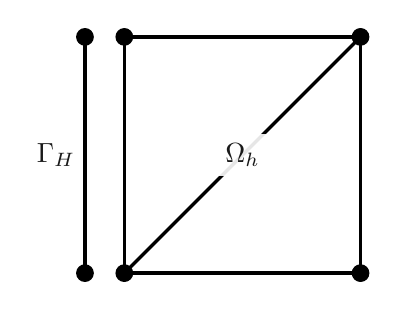
\begin{tikzpicture}
  \draw[black, very thick] (1,0) rectangle (4, 3);
  \draw[black, very thick] (1,0) -- (4, 3);
  \node[fill=white, opacity=0.9] at (2.5, 1.5) {$\Omega_{h}$};

  \node[mark size=3pt, color=black] at (1, 0) {\pgfuseplotmark{*}};
  \node[mark size=3pt, color=black] at (4, 0) {\pgfuseplotmark{*}};
  \node[mark size=3pt, color=black] at (1, 3) {\pgfuseplotmark{*}};
  \node[mark size=3pt, color=black] at (4, 3) {\pgfuseplotmark{*}};

  \draw[black, very thick] (0.5,0) -- (0.5, 3);
  \node[opacity=0.9, left] at (0.5, 1.5) {$\Gamma_{H}$};

  \node[mark size=3pt, color=black] at (0.5, 0) {\pgfuseplotmark{*}};
  \node[mark size=3pt, color=black] at (0.5, 3) {\pgfuseplotmark{*}};
\end{tikzpicture}
%
\hspace{50pt}
%
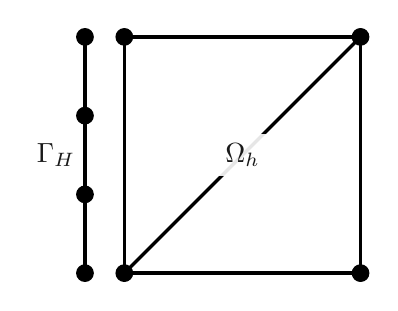
\begin{tikzpicture}
  \draw[black, very thick] (1,0) rectangle (4, 3);
  \draw[black, very thick] (1,0) -- (4, 3);
  \node[fill=white, opacity=0.9] at (2.5, 1.5) {$\Omega_{h}$};

  \node[mark size=3pt, color=black] at (1, 0) {\pgfuseplotmark{*}};
  \node[mark size=3pt, color=black] at (4, 0) {\pgfuseplotmark{*}};
  \node[mark size=3pt, color=black] at (1, 3) {\pgfuseplotmark{*}};
  \node[mark size=3pt, color=black] at (4, 3) {\pgfuseplotmark{*}};

  \draw[black, very thick] (0.5,0) -- (0.5, 3);
  \node[opacity=0.9, left] at (0.5, 1.5) {$\Gamma_{H}$};

  \node[mark size=3pt, color=black] at (0.5, 0) {\pgfuseplotmark{*}};
  \node[mark size=3pt, color=black] at (0.5, 1) {\pgfuseplotmark{*}};
  \node[mark size=3pt, color=black] at (0.5, 2) {\pgfuseplotmark{*}};  
  \node[mark size=3pt, color=black] at (0.5, 3) {\pgfuseplotmark{*}};
\end{tikzpicture}
%
\end{center}
  \caption{Two different settings considered for the Babu{\v s}ka problem
    \eqref{eq:bab}. Trace mesh (on $\Gamma_L$) of $\Omega_h$ equals (left)
    or differs (right) from $\Gamma_H$.
  }
\label{fig:domains}
\end{figure}


\subsection{Discretization by P1-P1 elements}\label{sec:p1_p1} We consider
finite element discretization of \eqref{eq:bab} in terms continuous linear
Lagrange elements (P1) for both spaces $V$ and $Q$.

\subsubsection{Matching case} We remark that Dirichlet boundary conditions
$p=0$ on $\partial\Gamma_L$ need to be enforced on the linear system in order
to obtain a non-singular system matrix. Then the discretization is inf-sup
stable as can be seen in Table \ref{tab:p1_p1} by observing that the MinRes
iterations using the Riesz map preconditioner remain bounded in the discretization
parameter. Note that the $Q$ block of (the diagonal) preconditioner represents
the action of the inverse of $-\Delta^{1/2}_{00}$. In particular, the fractional
operator is based on the eigenvalue problem
%
\[
\begin{aligned}
  -\Delta p &= \lambda p &\mbox{ in }\Gamma_L,\\
          p &= 0         &\mbox{ on }\partial\Gamma_L.
\end{aligned}
\]
%

\subsubsection{Non-matching case} Here $\dim Q_H$ is (considerably) larger
than the trace space of $V_h$ and stabilization of \cite{burman2014projection}
is needed to obtain inf-sup stability. More precisely, the discretization
of \eqref{eq:bab} reads: Find $u\in V_h$, $q\in Q_H$ such that
\[
\begin{aligned}
&\int_{\Omega} \nabla u\cdot \nabla v &+ \int_{\Gamma_L}p v &= \int_{\Omega} f v - \int_{\Gamma_N}h v &\forall v\in V_h,\\
  &\int_{\Gamma_L}q u  &-\gamma \sum_{K\in\Gamma_H}\int_{K} H_K^3\nabla p\cdot\nabla q &= \int_{\Gamma} g q &\forall q\in Q_H.
  \end{aligned}
\]
Here $\gamma$ is a stabilization parameter and we use $\gamma=1$ in the
following. As before, Dirichlet boundary conditions $p=0$ on $\partial\Gamma_L$ are
enforced.

MinRes iteration counts with the Riesz map preconditioner are shown in
Table \ref{tab:p1_p1}. Here, the $Q$ block of the preconditioner is
defined as
\[
\langle (-\Delta_{00})^{1/2} \bullet, q\rangle + \sum_{K\in\Gamma_H}\int_{K} H_K^3\nabla \bullet \cdot\nabla q,\quad q\in Q_H.
\]
%

\begin{table}
  \begin{center}
    \footnotesize{
  \begin{tabular}{c|cc|c|c||cc|c|c}
    \hline
    $h$ & $\norm{u-u_h}_1$ & $\norm{p-p_h}_0$ & \#{utters} & $\kappa$
        & $\norm{u-u_h}_1$ & $\norm{p-p_h}_0$ & \#{iters} & $\kappa$ \\
    \hline
8.84E-02 & 6.91E+00(--)   & 6.37E+00(--)   & 29 & 5.131 & 6.90E+00(--)  & 5.94E+00(--)    & 31 & 4.836\\
4.42E-02 & 3.54E+00(0.97) & 1.61E+00(1.98) & 26 & 5.176 & 3.54E+00(0.96) & 1.76E+00(1.75) & 29 & 4.846\\
2.21E-02 & 1.78E+00(0.99) & 5.45E-01(1.56) & 26 & 5.191 & 1.78E+00(0.99) & 5.95E-01(1.57) & 28 & 4.851\\
1.10E-02 & 8.93E-01(1.00) & 3.11E-01(0.81) & 25 & 5.195 & 8.93E-01(1.00) & 3.24E-01(0.88) & 26 & 4.853\\
5.52E-03 & 4.46E-01(1.00) & 2.12E-01(0.55) & 24 & 5.196 & 4.46E-01(1.00) & 2.16E-01(0.59) & 26 & 4.853\\
2.76E-03 & 2.23E-01(1.00) & 1.49E-01(0.51) & 24 & 5.196 & 2.23E-01(1.00) & 1.50E-01(0.52) & 24 & 4.854\\
1.38E-03 & 1.12E-01(1.00) & 1.06E-01(0.50) & 22 & --    & 1.12E-01(1.00) & 1.06E-01(0.51) & 22 & --   \\
    \hline
  \end{tabular}
  }
    \caption{Approximation errors, number of preconditioner MinRes iterations (\#) and
      condition number of the preconditioned problem \eqref{eq:bab} ($\kappa$) discretized
      with P1-P1 elements. (left) Matching case. (right) Non-matching case.}
  \label{tab:p1_p1}
  \end{center}
\end{table}
%
Concerning approximation properties of the discretization, note that the error
for the multiplier is reported in the $L^2$ norm and not the natural $H^{-1/2}$
norm. Nevertheless, the rate seems sub-optimal. This is likely due to the fact
that the multiplier in the manufactured test case does not satisfy the
Dirichlet boundary conditions employed in the discrete problem.

\subsection{Discretization by P1-P0 elements}\label{sec:p1_p0}
We consider finite element discretization of \eqref{eq:bab} in terms P1 elements
for the space $V$ while the multiplier space used piecewise constants elements
(P0). In both the matching and non-matching case the discretization is unstable
and inf-sup stability is obtained by using stabilization \cite{burman2014projection}.
That is, the disretization of \eqref{eq:bab} reads: Find $u\in V_h$, $q\in Q_H$ such that
\[
\begin{aligned}
&\int_{\Omega} \nabla u\cdot \nabla v &+ \int_{\Gamma_L}p v &= \int_{\Omega} f v - \int_{\Gamma_N}h v &\forall v\in V_h,\\
  &\int_{\Gamma_L}q u  &-\gamma \sum_{\mathcal{V}^0} \avg{H_K}^2\jump{p}\jump{q} &= \int_{\Gamma} g q &\forall q\in Q_H,
  \end{aligned}
\]
where $\mathcal{V}^0$ is the set of all interior vertices of $\Gamma_H$.

Table \ref{tab:p1_p0} shows stability and convergence properties of the approximation.
Note that the error in the multiplier converges linearly, cf. $\tfrac{1}{2}$ for
the P1-P1 discretization in Table \ref{tab:p1_p1}.

\begin{table}
  \begin{center}
    \footnotesize{
  \begin{tabular}{c|cc|c|c||cc|c|c}
    \hline
    $h$ & $\norm{u-u_h}_1$ & $\norm{p-p_h}_0$ & \#{iters} & $\kappa$
        & $\norm{u-u_h}_1$ & $\norm{p-p_h}_0$ & \#{iters} & $\kappa$ \\
    \hline
8.84E-02 & 6.88E+00(--)   & 2.83E+00(--)  & 26 & 4.749  & 6.91E+00(--)   & 1.17E+01(--)  & 35 & 6.940 \\
4.42E-02 & 3.54E+00(0.96) & 2.12E+00(0.42)& 28 & 4.817  & 3.54E+00(0.96) & 2.33E+00(2.33)& 35 & 6.973 \\
2.21E-02 & 1.78E+00(0.99) & 7.42E-01(1.51)& 28 & 4.840  & 1.78E+00(0.99) & 4.91E-01(2.24)& 30 & 6.987 \\
1.10E-02 & 8.93E-01(1.00) & 2.17E-01(1.78)& 25 & 4.850  & 8.93E-01(1.00) & 1.46E-01(1.75)& 28 & 6.994 \\
5.52E-03 & 4.46E-01(1.00) & 8.90E-02(1.28)& 23 & 4.853  & 4.46E-01(1.00) & 5.90E-02(1.31)& 27 & 6.996 \\
2.76E-03 & 2.23E-01(1.00) & 4.28E-02(1.06)& 23 & 4.853  & 2.23E-01(1.00) & 2.77E-02(1.09)& 26 & 6.995 \\
1.38E-03 & 1.12E-01(1.00) & 2.12E-02(1.01)& 23 & --     & 1.12E-01(1.00) & 1.36E-02(1.02)& 25 & --    \\  
    \hline
  \end{tabular}
    }
    \caption{Approximation errors, number of preconditioner MinRes iterations (\#) and
      condition number of the preconditioned problem \eqref{eq:bab} ($\kappa$) discretized
      with P1-P0 elements. (left) Matching case. (right) Non-matching case.}
  \label{tab:p1_p0}
  \end{center}
\end{table}

\section{Coupled multiscale problem}\label{sec:coupled} As a stepping stone
towards the coupled 3$d$-1$d$-1$d$ problem we consider first a coupled multiscale
problem where the dimensionality gap is 1. Given two bounded domains $\Omega^i \subset\mathbb{R}^2$,
$i=\left\{-, +\right\}$, let $\Gamma$ be the intersection of the domain boundaries,
cf. Figure \ref{fig:coupled_domain}. We are then interested in solving

\begin{minipage}{0.47\textwidth}
  \begin{equation}
    \begin{aligned}
      -\Delta u^i &= f &\mbox{ in }\Omega^{i}, i\in\left\{+, -\right\},\\
      u^i &= g^i &\mbox{ on }\partial\Omega^{i}\setminus\Gamma,\\
      \jump{u} &= 0 &\mbox{ on }\Gamma,\\
      -\Delta \hat{u} + \jump{\nabla u\cdot n}&= \hat{f} &\mbox{ on }\Gamma,\\
      \hat{u} &= \hat{g} &\mbox{ on }\partial\Gamma,\\
      u - \hat{u} &= g&\mbox{ on }\Gamma.\\
    \end{aligned}
\end{equation}
\null
\par\xdef\tpd{\the\prevdepth}
\end{minipage}
\hfill
\begin{minipage}{0.47\textwidth}
  \begin{figure}[H]
    \begin{center}
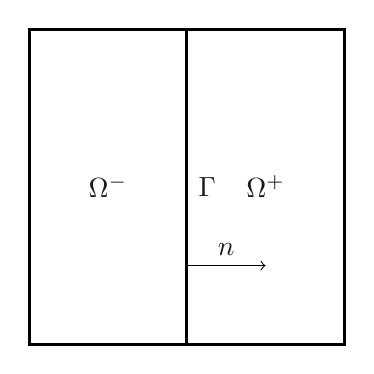
\begin{tikzpicture}
  \draw[black, very thick] (0,0) rectangle (4, 4);
  \draw[black, very thick] (2, 0) rectangle (2, 4);

  \node[fill=white, opacity=0.9] at (1, 2) {$\Omega^{-}$};
  \node[fill=white, opacity=0.9] at (3, 2) {$\Omega^{+}$};
  
  \draw[->, black] (2, 1) -- (3, 1);
  \node[fill=white, opacity=0.9, above] at (2.5, 1) {$n$};
  \node[fill=white, opacity=0.9, right] at (2.025, 2) {$\Gamma$};
\end{tikzpicture}
    \end{center}
    %\vspace{-20pt}
    \caption{Schematic domain coupled multiscale problem.}
    \label{fig:coupled_domain}
    %\vspace{5pt}    
\end{figure}
\end{minipage}
%


\bibliographystyle{siamplain}
\bibliography{stab}
\end{document}
